% !Mode:: "TeX:UTF-8"
\documentclass{xcumcmart}
\usepackage{setspace}
\usepackage{enumerate}
\usepackage{graphics}
\usepackage{tabu}

% \title{text}这里是显示在第三页的文章标题
\title{浅谈人工智能在医疗诊断中的应用}
% \author{何长鸿 2016141482154}

\linespread{1.5} %行距
\CTEXsetup[format={\Large\bfseries}]{section} %章节标题左对齐
\setlength{\parskip}{1.4em} %1.4倍段落距离

\begin{document}

\renewcommand\arraystretch{2}
\maketitle

\begin{abstract}
    \par 近年来由于深度学习的崛起,人工智能实现了巨大突破,相关技术正在逐渐渗透到各行各业。医疗诊断和辅助治疗为人工智能提供了巨大的舞台。而人工智能的特性及当下医疗行业的背景导致人工智能极其适合医疗诊断工作,人工智能在医学诊断中的应用具有极其重大的意义。为了更全面的了解人工智能的能力范围以及其在医学中的应用,与当前存在的一些不足。本文对人工智能以及肺癌诊断等人工智能诊断系统进行介绍,并对人工智能在医学诊断中的发展做出展望。
    \newline
    \par\textbf{关键词:人工智能 医学诊断 不足与展望}    
    \end{abstract}

\section{引言}
\par 在本学期的《医眼探秘》课程中,我们了解到了许多生理健康及高科技技术在医学诊断和治疗中的应用。作为一名计算机的学生,我对当前计算机前沿有一定了解,并结合我校的学科交叉的优势,对计算机与医学的交叉方向也有一定接触。在这里,我将对当下计算机前沿最热门的人工智能在医学中的研究进展、应用现状及发展展望做一些整理,并谈谈自己的理解。


\section{什么是人工智能?}
\par 人工智能(Artificial Intelligence),英文缩写为AI。它是研究、开发用于模拟、延伸和扩展人的智能的理论、方法、技术及应用系统的一门新的技术科学。人工智能是计算机科学的一个分支,它企图了解智能的实质,并生产出一种新的能以人类智能相似的方式做出反应的智能机器,该领域的研究包括机器人、语言识别、图像识别、自然语言处理和专家系统等\cite{1}。这里的专家系统,是一个智能计算机程序系统,其内部含有大量的某个领域专家水平的知识与经验,能够利用人类专家的知识和解决问题的方法来处理该领域问题。这也是人工智能在医学中发挥作用的最主要身份。
\par 深度学习是当下人工智能发展最快的一个分支,这是由于近年来硬件技术的提升,是的计算机有能力处理大规模数据,从而从数据提取特征构造分类预测模型。通俗的讲,人工智能系统发挥作用的必要条件是目前已经产生的大量数据,例如医学影像以及专家对于相应影像的诊断结果。科学家通过建模,从这些诊断结果和影像数据中学习其中的潜在关联因素,从而使得系统可以从新的医学影像中提取对应特征并给出判断结果。

\section{人工智能适合做什么?}

\par 临床上, 医学影像与常规疾病检查方法相结合, 逐渐成为医生做出医学诊断的重要依据。在此过程中, 医学影像数据的解读成为临床诊断中一项繁重且具有挑战的重要工作,目前, 医学影像数据中的信息仍然依靠知识全面、技术过硬的影像医生进行解读, 这种方式需要影像医生和临床医生的紧密配合, 并且具有以下4个方面缺点: (1) 诊断结果易受医生认知能力限制、主观因素干扰。 (2) 在影像数据的解读过程中, 医生随着疲劳程度增加, 极易误诊、漏诊。 (3) 现代医学影像数据结构复杂, 具有多样性。医生在提供个性化、精准诊疗方案等方面遇到巨大挑战。 (4) 多模态结合的影像大数据中潜藏着常规手段难以识别的深度信息。由此可见, 人工影像解读的方式已经难以为诊断提供足够信息。\cite{2}
\par 人工智能及其适合医疗诊断工作。上文已经说过,目前人工智能的主流是深度学习,而深度学习优秀的背后,是大量的病人的各种检查影像和生理指标和专家的诊断结果。换言之,我们可以通过对高水平医疗机构的数据进行学习构建专家系统,应用到缺乏相应资源的地方,从而减轻医疗机构的负担,提升其医疗水平。
\section{医学影像诊断}
\par 目前深度学习在医学领域已经有了多成功的应用,仅四川大学章毅教授实验室,就成功开发了乳腺智能诊断平台、眼科智能筛查平台、肺部智能诊断平台等多个高效的专家系统。以下以肺癌检测系统为例进行介绍。
\subsection{智能胸部疾病诊断系统}
\subsubsection{肺癌介绍}
国家癌症中心公布的最新数字显示,中国 2013 年恶性肿瘤发病率为 270.59/10 万,死亡率为 163.83/10 万,而肺癌在所有恶性肿瘤发病及死亡中均占首位,中国每年约 59.1 万人死于肺癌。肺癌是世界上发病率和死亡率最高的恶性肿瘤,而肺癌生存率与首次确诊时的疾病阶段高度相关,肺癌的早期发现和治疗,能够提高患者的生活质量和存活率。肺结节是早期肺癌的表现形式。因此,对肺结节的筛查尤其重要。
\begin{figure}[htbp]
        \centering
        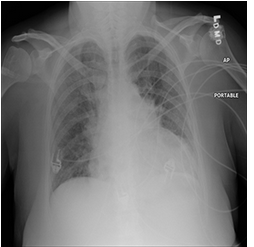
\includegraphics[width=0.6\textwidth,height=6cm]{fig/2.png}
        \caption{胸部X光影像\label{fig:alpy.jpeg}}
\end{figure}
  在临床上,早发现、早确诊、早治疗是降低肺结核和肺癌死亡率、提高患者生存率的关键措施。胸部 CT 放射影像技术,是肺癌早期筛查的有效手段,但一次检查会有多达数百张CT图像,医生仅用肉眼进行判断,费时费力。因此计算机辅助检测在减少医生工作量,帮助医生进行精确诊断方面表现出巨大的潜力。
\subsubsection{项目介绍}
\par 该项目利用当下最新的深度神经网络技术,使用公开数据集chestxray14,并联合华西医学院的雄厚医学背景,通过提出了一种新的损失层构建模型,显著地促进神经网络模型中深层网络的多标签分类训练,并实现包括肺癌在内的14种疾病的区分诊断。完成诊断后该系统还将自动生成诊断报告。 
\begin{figure}[htbp]
    \centering
    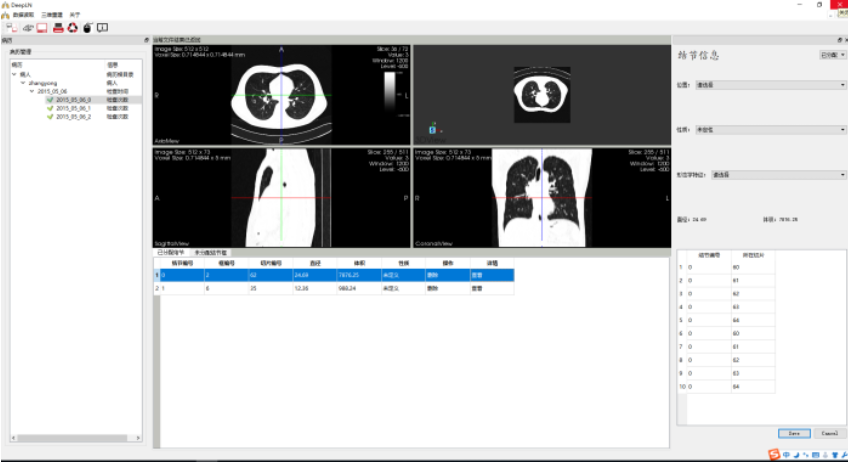
\includegraphics[width=0.6\textwidth,height=6cm]{fig/1.png}
    \caption{智能诊断系统\label{fig:py.jpeg}}
\end{figure}
\par “华西医院\&依图医疗”肺癌人工智能成果发布会暨互联网+医疗人工智能高端峰会上,双方合作研发的国内首个肺癌临床科研智能病种库和全球首个肺癌多学科智能诊断系统正式发布,其中的肺癌临床科研智能病种库,跨系统集成了2.8万例肺癌患者全周期数据,超过百万份临床文档和报告,超过千万份原始医学图像,收录肺癌患者的影像、病理、基因检测、病历文本等多维数据,也是国内首个基于人工智能技术的肺癌单病种科研数据库\cite{3}。
\par 基于人工智能技术的肺癌单病种科研数据库,打破了传统数据库无法同时纳入医院多个系统接口数据、单纯文本资料的局限,通过人工智能技术,对影像数据、基因数据、病理数据、文本数据等进行解析与重构,实现可视化、结构化,使科研数据提取效率成倍提升,大大减少了科研流程中的人力劳动,满足科研、临床、教学、管理等多场景的数据需求,为临床辅助、疾病研究、产品孵化等提供支持,其数据筛选准确率达到99.3\%。
\par 依托这个全球顶级的病种库高质量的医疗大数据基础,成功开发的全球首个肺癌多学科智能诊断系统,成为“最具医生思维”的AI应用,不仅能够实现结节筛查等初级功能,更能够实现肺癌全类型病灶的诊断覆盖,综合多学科临床信息进行综合诊断,其决策依据来源于国际、国内最新临床肺癌诊疗指南。
\section{智能诊断的总结与展望}
\par 首先, 人工智能系统的性能评估仍需改进。公用基准库是公平、正确衡量人工智能系统性能的基础。目前有些研究基于公用数据库的部分数据却没有说明选用数据的标准, 正确衡量系统性能非常困难。其次, 现阶段研究中监督学习占有重要比重, 但非监督学习更接近“智能”的本质。监督学习中海量数据的标注需要耗费大量人力、物力, 逐步提高现有研究中非监督学习的比重应成为未来发展方向。最后, 结果的可解释性是诊断值得信赖的前提。目前深度学习系统作为“黑盒”模型, 对结果的不理解限制了其临床应用, 由此可见, 结果解释性研究有待加强。
\par 虽然人工智能技术在医学影像诊断中的应用尚有不足, 但随着标准化与大样本数据中心的建立, 人工智能算法的发展, 量子计算机等硬件的突破, 人工智能和医学影像诊断的融合研究定能取得更大发展。

\begin{thebibliography}{1}
    \bibitem{1} 百度百科[EB/OL],人工智能 (计算机科学的一个分支),https://baike.baidu.com/item/人工智能/9180?fr=aladdin.
    \bibitem{2} 人工智能在医学影像诊断中的应用[J],刘丰伟、李汉军、张逸鹤、李若松、王尊升、唐晓英,背景生物医学工程,2019(02)。
    \bibitem{3} 四川大学综合新闻[EB/OL],四川大学华西医院与依图医疗联合开发的全球首个肺癌多学科智能诊断系统正式发布,http://www.scu.edu.cn/info/1207/4806.htm,2018,06/24.
\end{thebibliography}
\end{document}
